\documentclass[a4paper]{article}
\usepackage[a4paper,margin=0mm]{geometry}
\usepackage{fontspec}
\usepackage{unicode-math}
\usepackage{tikz}
\usepackage[table]{xcolor}
\usepackage[absolute]{textpos}
\usepackage{enumitem}
\usepackage{array}
\usepackage{multirow}

\setmainfont{Libertinus Serif}
\setsansfont{Libertinus Sans}
\setmathfont{Libertinus Math}
\newfontfamily\trackedsans{Libertinus Sans}[LetterSpace=8.0]

\definecolor{accent}{HTML}{F46530}
\definecolor{badge}{HTML}{FFBDA5}
\definecolor{ink}{HTML}{2A2E30}

\setlength{\TPHorizModule}{1mm}
\setlength{\TPVertModule}{1mm}
\setlength{\parindent}{0pt}
\pagestyle{empty}

\newcommand{\LCOL}{16mm}
\newcommand{\RCOL}{111mm}
\newcommand{\COLW}{83mm}

\newcommand{\topicheader}[2]{%
\begin{textblock*}{194mm}(16mm,10mm)
\begin{tikzpicture}
\node[fill=accent,text=white,font=\sffamily\bfseries\fontsize{13}{13}\selectfont,
      minimum width=9mm,minimum height=9mm,inner sep=0pt] at (4.5mm,-4.5mm) {#1};
\node[font=\sffamily\bfseries\fontsize{15}{16}\selectfont,text=ink,anchor=west] at (12mm,-4.5mm) {#2};
\end{tikzpicture}
\end{textblock*}
\begin{textblock*}{194mm}(16mm,22.5mm)

\begin{tikzpicture}
\fill[accent] (0,0) rectangle (194mm,0.5mm);
\end{tikzpicture}
\end{textblock*}
}

\newcommand{\pagefooter}[1]{%
\begin{textblock*}{194mm}(8mm,286.41mm)
  
\begin{tikzpicture}
    \fill[accent] (0,0) rectangle (194mm,0.6mm);
  \end{tikzpicture}
\end{textblock*}
\begin{textblock*}{63.59mm}(8mm,288.27mm)
  {\sffamily\bfseries\color{accent}\fontsize{13}{16}\selectfont SAT 1200+}
\end{textblock*}
\begin{textblock*}{10mm}(188mm,288.27mm)
  \centering{\sffamily\color{accent}\fontsize{14}{16}\selectfont #1}
\end{textblock*}
}

\newcommand{\colrule}[2]{%
\begin{textblock*}{1mm}(105mm,#1mm)
\begin{tikzpicture}
\draw[black!65,line width=0.5pt] (0,0) -- (0,#2mm);
\end{tikzpicture}
\end{textblock*}
}

\newcommand{\setkicker}[2]{%
{\sffamily\bfseries\fontsize{12}{14}\selectfont #1.}\ {\itshape\fontsize{11}{14}\selectfont\color{black!75} #2}\par\vspace{2mm}%
}

\setlength{\fboxsep}{1.4pt}
\setlength{\fboxrule}{0.5pt}
\newcommand{\pnum}[1]{\fcolorbox{ink}{white}{\sffamily\bfseries\fontsize{8}{8}\selectfont #1}~}

\newcommand{\qrbox}[1]{%
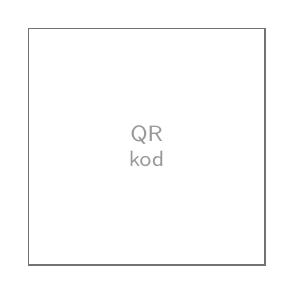
\begin{tikzpicture}
\draw[black!55,line width=0.6pt] (0,0) rectangle (30mm,30mm);
\node[black!40,font=\sffamily\fontsize{8}{9}\selectfont,align=center] at (15mm,15mm) {QR\\kod};
\end{tikzpicture}\\[1.5mm]
{\sffamily\fontsize{9}{11}\selectfont\color{black!70} #1}%
}

% ---- SAT-style multiple-choice question block: #1=number #2=stem #3-6=choices A-D ----
\newcommand{\satq}[6]{%
\noindent\pnum{#1} #2\\[2mm]
\hspace*{7mm}\begin{tabular}{@{}p{32mm}p{32mm}@{}}
(A) #3 & (B) #4 \\[2.5mm]
(C) #5 & (D) #6 \\
\end{tabular}\\[7mm]%
}

\arrayrulecolor{accent}
\setlength{\arrayrulewidth}{0.7pt}
\renewcommand{\arraystretch}{1.35}
\newcommand{\anstitle}[1]{{\sffamily\bfseries\color{accent}\fontsize{11}{13}\selectfont #1}\\[1.3mm]}

\begin{document}

% ================= PAGE 1: Set 1 | Set 2 =================
\topicheader{9}{Umumlashtiruvchi takrorlash}
\pagefooter{67}
\colrule{32}{238}
\mbox{}%

\begin{textblock*}{\COLW}(\LCOL,32mm)
{\fontsize{12}{15}\selectfont
\setkicker{1-to'plam}{Amallar tartibi va kasrlarni birlashtiring.}

\noindent\pnum{1} $\dfrac{3}{4}+2\times\!\left(\dfrac{1}{2}-\dfrac{1}{8}\right)=$\\[30mm]
\noindent\pnum{2} $\left(\dfrac{2}{3}+\dfrac{1}{6}\right)\times4-1=$\\[30mm]
\noindent\pnum{3} $10-3\times\!\left(\dfrac{2}{5}+\dfrac{1}{10}\right)=$\\[30mm]
\noindent\pnum{4} $\left(\dfrac{7}{8}-\dfrac{1}{4}\right)\div\dfrac{1}{2}=$\\[30mm]
\noindent\pnum{5} $2\times\dfrac{3}{4}+\left(1-\dfrac{1}{3}\right)\times6=$\\[30mm]
\noindent\pnum{6} $\left(\dfrac{1}{2}+\dfrac{1}{3}+\dfrac{1}{6}\right)\times12-5=$
}
\end{textblock*}

\begin{textblock*}{\COLW}(\RCOL,32mm)
{\fontsize{12}{15}\selectfont
\setkicker{2-to'plam}{Ishorali sonlar va darajalarni birlashtiring.}

\noindent\pnum{1} $(-2)^3-3\times(-4)=$\\[30mm]
\noindent\pnum{2} $-3^2+(-3)^2=$\\[30mm]
\noindent\pnum{3} $(-5)^2\div(-5)+2^3=$\\[30mm]
\noindent\pnum{4} $-2\times(-3)^2+(-4)=$\\[30mm]
\noindent\pnum{5} $(-1)^5\times(-2)^3=$\\[30mm]
\noindent\pnum{6} $4-(-2)^4\div2=$
}
\end{textblock*}

\clearpage

% ================= PAGE 2: Set 3 | Set 4 =================
\topicheader{9}{Umumlashtiruvchi takrorlash}
\pagefooter{68}
\colrule{32}{238}
\mbox{}%

\begin{textblock*}{\COLW}(\LCOL,32mm)
{\fontsize{12}{15}\selectfont
\setkicker{3-to'plam}{O'nli kasr/foiz va tenglamalarni birlashtiring. $x$ ni toping.}

\noindent\pnum{1} $0.25x+10=35$\\[30mm]
\noindent\pnum{2} $40\%$ of $x$ is $32$\\[30mm]
\noindent\pnum{3} $x-15\%$ of $x=68$\\[30mm]
\noindent\pnum{4} $0.5(x+4)=13$\\[30mm]
\noindent\pnum{5} $20\%$ of $(x+10)=16$\\[30mm]
\noindent\pnum{6} $x+0.1x=44$
}
\end{textblock*}

\begin{textblock*}{\COLW}(\RCOL,32mm)
{\fontsize{12}{15}\selectfont
\setkicker{4-to'plam}{Algebraik ifodalar va tenglamalarni birlashtiring. $x$ ni toping.}

\noindent\pnum{1} $3(x-2)+5=2x+7$\\[30mm]
\noindent\pnum{2} $2(x+3)-(x-1)=10$\\[30mm]
\noindent\pnum{3} $4x-(2x+5)=7$\\[30mm]
\noindent\pnum{4} $5(x-1)=3(x+3)$\\[30mm]
\noindent\pnum{5} $-2(x+4)+6=x-2$\\[30mm]
\noindent\pnum{6} $3(2x-1)-4=2(x+5)$
}
\end{textblock*}

\clearpage

% ================= PAGE 3: Set 5 | Set 6 =================
\topicheader{9}{Umumlashtiruvchi takrorlash}
\pagefooter{69}
\colrule{32}{238}
\mbox{}%

\begin{textblock*}{\COLW}(\LCOL,32mm)
{\fontsize{12}{15}\selectfont
\setkicker{5-to'plam}{Kasrli tenglamalarni yeching. $x$ ni toping.}

\noindent\pnum{1} $\dfrac{2}{3}x-1=5$\\[30mm]
\noindent\pnum{2} $\dfrac{x}{4}+3=7$\\[30mm]
\noindent\pnum{3} $\dfrac{3}{4}x+\dfrac{1}{2}=2$\\[30mm]
\noindent\pnum{4} $\dfrac{x+2}{3}=5$\\[30mm]
\noindent\pnum{5} $\dfrac{2x-1}{5}=3$\\[30mm]
\noindent\pnum{6} $\dfrac{x}{2}-\dfrac{x}{3}=2$
}
\end{textblock*}

\begin{textblock*}{\COLW}(\RCOL,32mm)
{\fontsize{12}{15}\selectfont
\setkicker{6-to'plam}{$f(x)$ funksiyasi, ishorali sonlar va darajalar.}

\noindent\pnum{1} $f(x)=-2x^2+3$. $f(-2)=$\\[26mm]
\noindent\pnum{2} $f(x)=x^3-4x$. $f(-1)=$\\[26mm]
\noindent\pnum{3} $f(x)=(x-2)^2$. $f(-3)=$\\[26mm]
\noindent\pnum{4} $f(x)=2x^2-5x+1$. $f(-1)=$\\[26mm]
\noindent\pnum{5} $f(x)=-x^2+2x$. $f(3)=\ ?\quad f(-3)=$\\[26mm]
\noindent\pnum{6} $f(x)=kx+b$. $f(2)=7$, $f(0)=3$. $k=\ ?\quad b=$
}
\end{textblock*}

\clearpage

% ================= PAGE 4: Set 7 (spot the error) | Set 8 (bonus) =================
\topicheader{9}{Umumlashtiruvchi takrorlash}
\pagefooter{70}
\colrule{32}{238}
\mbox{}%

\begin{textblock*}{\COLW}(\LCOL,32mm)
{\fontsize{11}{14}\selectfont
\setkicker{7-to'plam}{Xatoni toping -- ikki mavzu aralashgan, bitta xato qadam bor.}

\noindent\pnum{1} $\dfrac12x+3=7$ ifodasida ko'rsatilgan yechimda xato bor:\\[1mm]
\hspace*{7mm}\textit{``$\frac12x=7+3=10$, shuning uchun $x=20$.''}\\[2mm]
\hspace*{7mm}Xato va to'g'ri javob: \makebox[52mm]{\dotfill}\\[8mm]

\noindent\pnum{2} $3(x-2)=9$ ifodasida ko'rsatilgan yechimda xato bor:\\[1mm]
\hspace*{7mm}\textit{``$3x-2=9$, shuning uchun $3x=11$, $x=\frac{11}{3}$.''}\\[2mm]
\hspace*{7mm}Xato va to'g'ri javob: \makebox[52mm]{\dotfill}\\[8mm]

\noindent\pnum{3} $f(x)=x^2-2x$, $f(-3)$ ifodasida ko'rsatilgan yechimda xato bor:\\[1mm]
\hspace*{7mm}\textit{``$f(-3)=(-3)^2-2(-3)=9-6=3$.''}\\[2mm]
\hspace*{7mm}Xato va to'g'ri javob: \makebox[52mm]{\dotfill}\\[8mm]

\noindent\pnum{4} $0.4x=24$ ifodasida ko'rsatilgan yechimda xato bor:\\[1mm]
\hspace*{7mm}\textit{``$x=24\times0.4=9.6$.''}\\[2mm]
\hspace*{7mm}Xato va to'g'ri javob: \makebox[52mm]{\dotfill}\\[8mm]

\noindent\pnum{5} $2(x+1)-x=9$ ifodasida ko'rsatilgan yechimda xato bor:\\[1mm]
\hspace*{7mm}\textit{``$2x+1-x=9$, $x+1=9$, $x=8$.''}\\[2mm]
\hspace*{7mm}Xato va to'g'ri javob: \makebox[52mm]{\dotfill}
}
\end{textblock*}

\begin{textblock*}{\COLW}(\RCOL,32mm)
{\fontsize{12}{15}\selectfont
\setkicker{8-to'plam}{Bonus / eng qiyin -- bitta masalada 3+ ko'nikma.}

\noindent\pnum{1} $\dfrac12(x-4)+0.25x=5$\\[34mm]
\noindent\pnum{2} $f(x)=-2(x-1)^2+3$. $f(-1)=$\\[34mm]
\noindent\pnum{3} $30\%$ of $(2x+10)=x+2$\\[34mm]
\noindent\pnum{4} $\dfrac34x-(-2)^3=11$\\[34mm]
\noindent\pnum{5} $f(x)=kx+b$. $f(-2)=1$, $f(2)=9$. $k=\ ?\ b=\ ?\ f(0)=$
}
\end{textblock*}

\clearpage

% ================= PAGE 5: Set 9 (SAT-style application, MC) -- own page =================
\topicheader{9}{Umumlashtiruvchi takrorlash}
\pagefooter{71}
\colrule{32}{238}
\mbox{}%

\begin{textblock*}{\COLW}(\LCOL,32mm)
{\fontsize{10.5}{13}\selectfont
\setkicker{9-to'plam}{SAT'da qanday uchraydi -- 1--8-darslarning barchasidan.}

\satq{1}{$3+2\times(7-4)^2$ ifodaning qiymati nechaga teng?}{15}{21}{30}{45}
\satq{2}{Retseptda $\frac34$ stakan shakar kerak. Retseptning $\frac23$ qismini tayyorlash uchun necha stakan shakar kerak?}{$\frac{5}{12}$}{$\frac12$}{$\frac34$}{$\frac23$}
\satq{3}{Ko'ylak \$40 turadi va 25\% chegirma bilan sotilmoqda. Chegirmali narx nechaga teng?}{\$10}{\$15}{\$30}{\$35}
\satq{4}{$(-4)+(-3)\times(-2)$ ifodaning qiymati nechaga teng?}{$-10$}{$-2$}{2}{14}
\satq{5}{$3(2x-1)-(x+4)$ ifodasiga teng ifodani toping.}{$5x-7$}{$5x+7$}{$7x-7$}{$2x-7$}
\satq{6}{$4x-5=2x+9$ tenglamasini qanoatlantiruvchi $x$ qiymatini toping.}{2}{5}{7}{9}
}
\end{textblock*}

\begin{textblock*}{\COLW}(\RCOL,32mm)
{\fontsize{10.5}{13}\selectfont
\vspace{9mm}

\satq{7}{$2^3\times2^2$ ifodaning qiymati nechaga teng?}{10}{16}{32}{64}
\satq{8}{Agar $f(x)=2x-5$ bo'lsa, $f(4)$ nechaga teng?}{$-1$}{3}{8}{13}
\satq{9}{$\dfrac12+\dfrac34\times2$ ifodaning qiymati nechaga teng?}{1}{$\frac54$}{$\frac32$}{2}
\satq{10}{$-20$ va $16$ sonlari yig'indisining 50\%-i nechaga teng?}{$-18$}{$-2$}{2}{18}
\satq{11}{$x>0$ bo'lsa, $x^2=49$ tenglamasini qanoatlantiruvchi $x$ nechaga teng?}{7}{$-7$}{24.5}{98}
\satq{12}{Agar $f(x)=-x^2+3$ bo'lsa, $f(-2)$ nechaga teng?}{$-7$}{$-1$}{1}{7}
}
\end{textblock*}

\clearpage

% ================= PAGE 6: Javoblar -- unified answer table + QR =================
\topicheader{9}{Umumlashtiruvchi takrorlash}
\pagefooter{72}
\mbox{}%

\begin{textblock*}{194mm}(16mm,30mm)
{\bfseries\itshape\color{accent}\fontsize{19}{21}\selectfont\centering Javoblar\par}
\end{textblock*}

\begin{textblock*}{194mm}(16mm,44mm)
{\fontsize{9.3}{11.6}\selectfont
\centering
\renewcommand{\arraystretch}{1.25}
\begin{tabular}{|>{\centering\arraybackslash}p{24mm}|>{\centering\arraybackslash}p{9mm}|>{\centering\arraybackslash}p{29mm}|>{\centering\arraybackslash}p{9mm}|>{\centering\arraybackslash}p{29mm}|}
\hline
\rowcolor{badge!55}\textbf{To'plam} & \textbf{\#} & \textbf{Javob} & \textbf{\#} & \textbf{Javob}\\
\hline
\multirow{3}{24mm}{\centering 1-to'plam} & 1 & $\frac32$ & 2 & $\frac73$\\\cline{2-5}
 & 3 & $\frac{17}{2}$ & 4 & $\frac54$\\\cline{2-5}
 & 5 & $\frac{11}{2}$ & 6 & $7$\\\hline
\multirow{3}{24mm}{\centering 2-to'plam} & 1 & 4 & 2 & 0\\\cline{2-5}
 & 3 & 3 & 4 & $-22$\\\cline{2-5}
 & 5 & 8 & 6 & $-4$\\\hline
\multirow{3}{24mm}{\centering 3-to'plam} & 1 & $x{=}100$ & 2 & $x{=}80$\\\cline{2-5}
 & 3 & $x{=}80$ & 4 & $x{=}22$\\\cline{2-5}
 & 5 & $x{=}70$ & 6 & $x{=}40$\\\hline
\multirow{3}{24mm}{\centering 4-to'plam} & 1 & $x{=}8$ & 2 & $x{=}3$\\\cline{2-5}
 & 3 & $x{=}6$ & 4 & $x{=}7$\\\cline{2-5}
 & 5 & $x{=}0$ & 6 & $x{=}\frac{17}{4}$\\\hline
\multirow{3}{24mm}{\centering 5-to'plam} & 1 & $x{=}9$ & 2 & $x{=}16$\\\cline{2-5}
 & 3 & $x{=}2$ & 4 & $x{=}13$\\\cline{2-5}
 & 5 & $x{=}8$ & 6 & $x{=}12$\\\hline
\multirow{3}{24mm}{\centering 6-to'plam} & 1 & $-5$ & 2 & $3$\\\cline{2-5}
 & 3 & $25$ & 4 & $8$\\\cline{2-5}
 & 5 & \multicolumn{3}{p{67mm}|}{$f(3){=}{-}3$, $f(-3){=}{-}15$}\\\cline{2-5}
 & 6 & \multicolumn{3}{p{67mm}|}{$k{=}2$, $b{=}3$}\\\hline
\multirow{5}{24mm}{\centering 7-to'plam} & \multicolumn{4}{p{77mm}|}{1.\ Teskari amal xato -- $3$ qo'shish o'rniga ayirish kerak edi. To'g'ri: $\frac12x=4$, $x=8$.}\\\cline{2-5}
 & \multicolumn{4}{p{77mm}|}{2.\ $3$ faqat $x$ ga taqsimlangan, $-2$ ga emas. To'g'ri: $3x-6=9$, $x=5$.}\\\cline{2-5}
 & \multicolumn{4}{p{77mm}|}{3.\ $-2\times(-3)=-6$ emas, $+6$. To'g'ri: $9+6=15$.}\\\cline{2-5}
 & \multicolumn{4}{p{77mm}|}{4.\ Ko'paytirish o'rniga bo'lish kerak edi. To'g'ri: $x=24\div0.4=60$.}\\\cline{2-5}
 & \multicolumn{4}{p{77mm}|}{5.\ $2$ faqat $x$ ga taqsimlangan, $+1$ ga emas. To'g'ri: $2x+2-x=9$, $x=7$.}\\\hline
\multirow{3}{24mm}{\centering 8-to'plam} & 1 & \multicolumn{3}{p{67mm}|}{$x{=}\frac{28}{3}$}\\\cline{2-5}
 & 2 & $-5$ & 3 & $x{=}\frac52$\\\cline{2-5}
 & 4 & $x{=}4$ & 5 & \multicolumn{1}{p{29mm}|}{$k{=}2,b{=}5$}\\\hline
\multirow{6}{24mm}{\centering 9-to'plam} & 1 & B & 2 & B\\\cline{2-5}
 & 3 & C & 4 & C\\\cline{2-5}
 & 5 & A & 6 & C\\\cline{2-5}
 & 7 & B & 8 & B\\\cline{2-5}
 & 9 & D & 10 & B\\\cline{2-5}
 & 11 & A & 12 & B\\\hline
\end{tabular}
}
\end{textblock*}

\begin{textblock*}{194mm}(16mm,225mm)
\centering
{\sffamily\fontsize{9.5}{11.5}\selectfont\color{black!70} Video yechimlar va qo'shimcha testlar uchun quyidagi QR kodlarni skanerlang:}\\[4mm]
\begin{minipage}[t]{32mm}\centering\qrbox{YouTube}\end{minipage}%
\hspace{16mm}%
\begin{minipage}[t]{32mm}\centering\qrbox{Telegram}\end{minipage}
\end{textblock*}

\end{document}
